\documentclass{beamer}
\usetheme{metropolis}
\usepackage{graphicx}
\usepackage{subfig}
\usepackage{hyperref}
\usepackage{tcolorbox}
\title{Calculus-Based Physics-1: Mechanics (PHYS150-01): Week 4}
\date{September 25th - September 29th, 2017}
\author{Jordan Hanson}
\institute{Whittier College Department of Physics and Astronomy}

\begin{document}
\maketitle

\section{Week 3 Review}

\begin{frame}{Week 3 Review}
\begin{enumerate}
\item Displacement, velocity and acceleration vectors \alert{as functions of time}
\begin{itemize}
\item Breaking into components
\item Derivatives of components
\end{itemize}
\item Combining free-fall and vector components: \alert{projectile motion}
\begin{itemize}
\item The independence of velocity components
\item \textbf{Lab-activity: testing component independence}
\end{itemize}
\item Relative motion and reference frames
\begin{itemize}
\item Relative motion in one-dimension
\item Relative motion in two-dimensions
\end{itemize}
\end{enumerate}
\end{frame}

\section{Week 3 Review Problems}

\begin{frame}{Week 3 Review Problems}
\small
A pilot is performing an airdrop maneuver, in which he must release a package of supplies to land on a beach.  The plane is traveling towards the beach at a speed of 100 kilometers per hour, with an altitude of 500 meters.  How far offshore must the pilot release the supplies such that the package lands on the sandy beach and not in the water?
\begin{itemize}
\item A: 280 m 
\item B: 410 m
\item C: 100 m
\item D: 170 m
\end{itemize}
\end{frame}

\begin{frame}{Week 3 Review Problems}
\small
Suppose the pilot is flying straight, adjusting for a cross-wind of 3 m/s.  How far to the side of the flight path of the plane does the package land, assuming the package is released 280 m from the shore?
\begin{itemize}
\item A: 10.1 seconds
\item B: 5.4 seconds
\item C: 3.2 seconds
\item D: 1.1 seconds
\end{itemize}
\end{frame}

\section{Week 4 Summary}

\begin{frame}{Week 4 Summary}
\begin{figure}
\centering
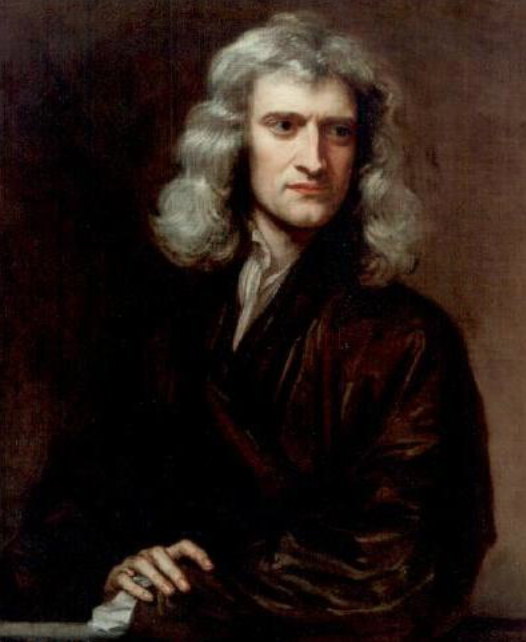
\includegraphics[width=0.5\textwidth]{figures/newton.png}
\caption{\label{fig:newton} A portrait of Sir Isaac Newton.}
\end{figure}
\end{frame}

\begin{frame}{Week 4 Summary}
\begin{enumerate}
\item Deep statements about physics: \textit{dynamics} and \textit{kinematics}
\begin{itemize}
\item \textbf{Lab activity}: Force, mass and stretching springs
\end{itemize}
\item Newton's \alert{First Law}
\item Newton's \alert{Second Law}
\item Newton's \alert{Third Law}
\item Applications
\begin{itemize}
\item Free-body diagrams
\item Tension
\item Inclined surfaces
\item Restoring forces
\end{itemize}
\end{enumerate}
\end{frame}

\begin{frame}{Deep statements about physics: dynamics and kinematics}
\small
\textit{Kinematics} - A \alert{description} of the motion of particles and systems \\
\textit{Dynamics} - An \alert{explanation} of the motion of particles and systems \\
\vspace{0.25cm}
What causes an object to move?  \textbf{Forces}.  Forces exist as a result of the \alert{\textbf{interactions}} of objects or systems.\\
\vspace{0.25cm}
\rule{10cm}{0.4pt} \\
\vspace{0.25cm}
\textit{Evolution} - A \alert{description} of the change of biological species \\
\textit{Natural Selection} - An \alert{explanation} of change in biological species \\
\vspace{0.25cm}
What causes species to evolve?  \textbf{Natural selection}.  Natural selection exists because of \alert{election pressures}, \alert{numerous offspring}, and \alert{variation} among offspring.
\end{frame}

\begin{frame}{What is a force, in practice?}
A force has units of \textit{Newtons}, just like distance has units of \textit{meters}.  One Newton is the force required to make an object of mass 1 kilogram accelerate by 1 m/s$^2$.\\
\vspace{1cm}
A force must also be a \textit{vector}: if a force acts on a system in a certain direction, the object will accelerate in that direction. \\
\vspace{1cm}
Force has to be related to mass in some way.
\end{frame}

\begin{frame}{What is a force, in practice?}
\small
\begin{figure}
\centering
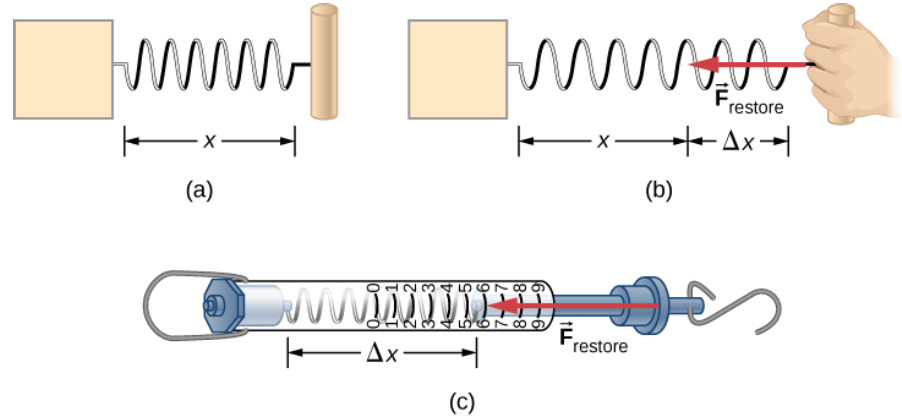
\includegraphics[width=0.9\textwidth]{figures/force1.png}
\caption{\label{fig:force1} (a) No interaction is stretching the spring.  (b) An interaction stretches the spring a distance $\Delta x$, and the spring pulls back.  (c) A device that can compare forces by comparing $\Delta x$ for different interactions (connecting to different weights, for example).}
\end{figure}
\end{frame}

\begin{frame}{What is a force, in practice?}
\textbf{Lab activity}: Force, mass, and stretched springs.
\begin{enumerate}
\item Obtain a set of weights, a force-meter (spring), and a ruler.
\item Hang a weight from the spring, and measure the extra distance the spring stretches.
\item Repeat with different weights, recording the stretched distances alongside the weights.
\item Compute the ratio of the mass of the weight to the stretched distance in each case.  What is the result?
\end{enumerate}
\end{frame}

\begin{frame}{What is a force, in practice?}
Thus, if a force causes \textit{a system with some mass} to accelerate, the force must be \textit{proportional to that mass}.  \alert{``If it is heavier, we mush push it harder, to obtain the same acceleration.''}  \\
\vspace{1cm}
Now, let's consider all the systems for which we have described the \textit{kinematics}, where we made no use of the concept of a force...
\end{frame}

\section{Newton's First Law}

\begin{frame}{Newton's First Law}
\begin{tcolorbox}[colback=white,colframe=red!40!blue,title=Newton's First Law]
\alert{A body at rest remains at rest or, if in motion, remains in motion at constant velocity unless acted on by a net external force.}
\end{tcolorbox}
\end{frame}

\begin{frame}{Newton's First Law}
\small
For most people in the late 15th and early 16th centuries, Newton's First Law was not intuitive.  ``When have you ever seen a thing move perpetually?''\\
\vspace{0.5cm}
The key is the last phrase: ``\textit{...unless acted on by a \alert{net} external force}.''  Nothing moves unless forced, and if the \alert{net} force is zero, the velocity does not change.  Thus, if some object has a constant velocity, then it remains at that velocity unless some force (friction, air-resistance, gravity, a wall) interrupts. \\
\vspace{0.5cm}
\url{https://openstaxcollege.org/l/21forcemotion}
\end{frame}

\section{Conclusion}

\section{Answers}

\begin{frame}{Answers}
\begin{columns}[T]
\begin{column}{0.5\textwidth}
\begin{itemize}
\item 280 m
\item 10.1 seconds
\end{itemize}
\end{column}
\begin{column}{0.5\textwidth}
\begin{itemize}
\item
\end{itemize}
\end{column}
\end{columns}
\end{frame}

\end{document}
